\chapter{Research Methodology}

	This chapter outlines and expands upon the research methodology for the design and implementation of a shelter location-allocation system using a genetic algorithm for the optimization of shelter placement in disaster-prone areas. This methodology provides a systematic approach for a clear framework for system design, model implementation, and evaluation. Following this, data collection procedures are explained including the sources and techniques for gathering essential data on community demographics, geographic information, and shelter facilities.
	
	Additionally, this chapter addresses the criteria for selecting, cleaning, and analyzing data, as well as the metrics used to evaluate the system’s acceptability. Finally, ethical considerations such as data privacy are also discussed.

\section{Research Design}
	The research design for this study is mixed-method applied research, this approach combines both quantitative and qualitative methods to provide a structured framework for development and evaluation of the shelter location allocation system.

\subsection{Applied Research}
	The applied research aspect of this study focuses on developing and implementing a practical solution for shelter location-allocation in real-world scenarios. The primary objective is to create a shelter location-allocation system using a genetic algorithm.
	This applied research approach aims to deliver a functional and reliable shelter location-allocation system that local government units (LGUs) and disaster response agencies can easily deploy and adapt. By emphasizing incremental progress and user-centered development, this ensures that the research outputs are directly applicable and beneficial to communities in disaster-prone areas.

\subsection{Quantitative Research}
	The quantitative research component of this study aims to measure and analyze the acceptability of the proposed system using TAM determinants and ISO/IEC 25010 standard. The approach provided objective and measurable evidence to evaluate the system's usability, reliability, and overall quality performance. The quantitative methods quantify the use of genetic algorithms in the shelter location allocation system, providing valuable insights into the system's effectiveness for emergency management.
	Methods included collecting user feedback and performance metrics through structured surveys and system testing to assess these attributes. The survey has gauged user satisfaction with system usability and functionality using a 10-point rating scale, providing quantifiable insights into the system's ease of use and accessibility. 
	Incorporating quantitative research in this study is justified as it can provide empirical evidence supporting the shelter allocation system's acceptability. 

\subsection{Qualitative Research}
	The researchers used qualitative research to understand the current issues of shelter location allocation from the stakeholders' perspectives. This approach requires engaging with the LGU offices to identify the additional requirements for the system. This ensured that the development of the shelter location-allocation system addresses real-world challenges and support those involved in evacuating communities during natural disasters and be of acceptable quality.
	The researchers has conducted an interview to achieve this. The interview was based on Decision Thinking Framework which is a common framework for developing a product. This was chosen to provide a structured way to gather detailed feedback from the stakeholders about their experiences, challenges, information about the shelters, and expectations regarding shelter location-allocation and this study. This method allows the researchers to collect various opinions and insights, which is important for understanding the complex issues involved in disaster management and shelter allocation.
	This insight is important for ensuring the system's effectiveness, as it helps identify the challenges to ensure the proper functioning of the shelter location allocation system and meet the needs of the affected communities. By capturing these detailed perspectives, the system is more practical, user-friendly, and responsive to the real-world needs of disaster management.

\section{Model Adoption}
	The model adopted for this study is the Bilevel No-transfer (BNT) Model, which solves the shelter location-allocation problem under disaster scenarios. As discussed in a published paper by \textcite{LeahUP}, this model is effective when it assigns communities to shelters without allowing transfers between different shelter levels during recovery. Using the BNT Model, the researchers can optimize the allocation of communities to shelters, accounting for each shelter’s capacity and travel distance for evacuees.
	The BNT Model includes a two-tiered shelter structure, consisting of level 1 and 2 shelters. Level 1 shelters are smaller facilities intended for immediate use, providing basic services for short-term stays. In contrast, Level 2 shelters are significantly larger and equipped with comprehensive services, including private rooms and extended support amenities, these shelters are intended for longer-term stays. However, once assigned to a shelter in the BNT Model, evacuees remain in that shelter until the disaster subsides, eliminating the need for transfers between shelters.
	The objective function for the BNT model can be expressed as follows:
	
	Minimize 
	\begin{equation}
		wt_{dist}\sum_{j=1}^{N}\sum_{i=1}^{M}d_{ij}P_{i}x_{ij}+wt_{cost}\sum_{k=1}^{2}\sum_{j=1}^{N}C_{j}^{(k)}y_{j}^{(k)} 
	\end{equation}
	
	The constraints of BNT model include the distance, capacity, assignment, and binary constraints, each of which plays a crucial role in ensuring the model functions effectively under the disaster response scenario. These constraints subject to the following: 
	
	\textit{Distance Constraint.} Equation \ref{c1} ensures that each community is allocated to a shelter within a defined maximum distance. 
	\begin{equation} 	
		\label{c1}
		d_{ij}x_{ij} \le D_{i}, \forall i = 1,..., M,  \forall j = 1,..., N 
	\end{equation}
	
	\textit{Capacity Constraint.} Equation \ref{c2} guarantees that the total number of evacuees assigned to a shelter does not exceed its maximum capacity. 
	\begin{equation} 
		\label{c2}
		\sum_{i=1}^{M}LP_{i}x_{ij} \le \sum_{k} Area_{j}^{(k)} y_{j}^{(k)}, \forall j = 1,..., N , k=1,2
	\end{equation}
	
	\textit{Assignment Constraints.} Equations \ref{c3} and \ref{c4} ensures that the total assigned shelters and level 2 shelter does not exceeds over the user defined parameters respectively.  Equation \ref{c5} ensures that every community is assigned to exactly one shelter. Equation \ref{c6} ensures that the assigned shelter does not duplicate like being opened as level 1 and level 2 at the same time. This prevents problems in shelter allocation and ensures that each community has a designated place.
	\begin{equation} 
		\label{c3}
		\sum_{k=1}^{2} \sum_j={1}^{N}y_{j}^{(k)} \le MaxSh
	\end{equation}
	\begin{equation}
		\label{c4} 
		\sum_j={1}^{N}y_{j}^2 \le MaxL2
	\end{equation}
	\begin{equation}
		\label{c5}
		\sum_{j=1}^{N}x_{ij} = 1, \forall i=1,...,M
	\end{equation}
	\begin{equation}
		\label{c6}
		\sum_{k=1}^{N}y_{j}^{(k)} \le 1, \forall j=1,...,N
	\end{equation}\\
	
	
	\textit{Binary Constraint.} Equation \ref{c7} ensures that the model only takes binary variable, where can either be true (1) or false (0)
	\begin{equation}
		\label{c7}
	 	x_{ij}, y_{j}^{(1)},y_{j}^{(2)} \in \{0,1\}, \forall i=1,...,M,  \forall j=1,...,N
	\end{equation}
	
	\noindent where: \\
	\begin{tabular}{@{}ll}
	$wt_{dist}$ & weight given to the distance cost. \\
	$wt_{cost}$ & weight given to the fixed shelter cost. \\
	$M$ & total number of communities. \\
	$N$ & total number of potential shelter locations. \\
	$d_{ij}$ & distance between shelter $i$ and community $j$. \\
	$P_{i}$ & population of community $i$. \\
	$C_{j}^{(k)}$ & fixed cost for establishing shelter $j$ of level $k$. \\
	$x_{ij}$ & binary decision variable indicating if community $j$ is assigned to shelter $i$. \\
	$y_{j}^{(k)}$ & binary decision variable indicating if shelter $j$ of level $k$ is opened. \\
	$L$ & area allotted per individual. \\
	$D_{i}$ & maximum distance that community $i$ can be traveled. \\
	$Area_{j}^{(k)}$ & area of shelter $j$ of level $k$. \\
	$MaxL2$ & maximum number of level 2 shelters to be opened. \\
	$MaxSh$ & maximum number of shelters to be opened. \\
	\end{tabular}
	
	
	
\subsection{Feasibility Conditions}

	Checking if a solution exists based on the user defined parameters is a must in developing the system thus conducting feasibility checks before executing the algorithm. This adds a feature that allows users to view if their inputs are incorrect having an additional functionality and capability of the system.
	
	The following conditions should satisfy else no solution exists:
	\begin{equation*} 
		\label{f1}
		Area_{j}^{(2)} \ge Area_{j}^{(1)}, \forall j = 1, ..., N
	\end{equation*}
	checks if shelter j area for level 2 is greater than or equal to their area for level 1. 
	\begin{equation*} 
		\label{f2}
		MaxL2 \le MaxSh
	\end{equation*}
	checks if the user defined number of maximum level 2 shelters is less than to number of maximum shelters.
	\begin{equation*} 
		\label{f3}
		\exists j \in d_{ij} \le D_{i}, \forall i = 1, ..., M
	\end{equation*}
	checks if there exists a distance from community i to all shelters that is less than or equal to its max distance.
	\begin{equation*} 
		\label{f4}
		\exists i \in LP_{i} \le Area_{j}^{(2)}, \forall j = 1, ..., N
	\end{equation*}
	checks if there exists a level 2 shelter that could accommodate a community i by their population multiplied by the area allotted per individual. 
	\begin{equation*} 
		\label{f5}
		\sum_{i=1}^{M}P_{i} \le L\sum_{j=1}^{N}Area_{j}, \forall i=1,...,M,  \forall j=1,...,N
	\end{equation*}
	checks if the total population is less than or equal to the total area of shelters multiplied to area allotted per individual. If this fails, then it is theoretically impossible to allocate all individuals given with their shorted capacity of shelters.
	
	Incorporating these feasibility conditions ensures that the model produced at least one feasible solution, and the system proceeds only with valid input configurations. By verifying these conditions, users receive instant feedback on whether their inputs are valid, allowing the model to proceed with solving. These conditions represent key feasibility checks but are not exhaustive, and infeasible solutions may still persist. An additional feature would employ a penalty function that would transform the model to an unconstrained model.	
	
\subsection{Penalty Function}
	The penalty function was used to handle the problem constraints. Instead of discarding infeasible solutions or chromosomes, they are assigned a very large objective value making them not fit to be a solution. The type of penalty to be used is the Courant-Beltrami penalty function method, as shown in equation
	\begin{equation*} 
		\label{p1}
		h(x)=(g^+(x))^2
	\end{equation*}
	where
	\begin{equation*} 
		\label{p2}
		g^+(x)=max\{g(x),0\}
	\end{equation*}
	where $g(x)$ is a constraint function of the form $g(x)\le0$. 
	\\
	
	The new objective function would be adding the initial objective value $f(x)$ to the penalty multiplied by some constant $\gamma$.
	\begin{equation*} 
		\label{p3}
		f_{new}(x)=f(x)+\gamma\sum_{i=1}^{n}(max\{g_i(x),0\})^2
	\end{equation*}
	
	where $g_1(x),g_2(x),...g_n(x)$ are the constraints of the model of the form $g_i(x)\le0$, and $\gamma\in\mathbb{R}^+$ is sufficiently large, where for this thesis is set to $10^{20}$. The penalty would add up to the objective value for each constraints it violated, otherwise it would not affect the objective value.	
	
\subsection{Optimization Technique}
	In a study created by \textcite{Mathew2012}, Genetic Algorithms are based on the concept of natural selection and evolves possible solutions through operators such as selection, crossover, and mutation. This algorithm iteratively evolved a population of potential solutions, utilizing operations to explore the population space and gradually converge toward an optimal solution.
	
	The BNT model was originally solved using Binary Genetic Algorithm implemented in MATLAB. However, since system integration was conducted on this thesis, the model has been solved using Integer-based Genetic Algorithm implemented in Python. This decision derived for satisfying the assignment constraint of the model, and Python being a well suited programming language for both data simulation and system development.
	
	The researchers start by defining some terms of genetic algorithm that are used in the context of shelter location-allocation model.
	
	\textit{Chromosome.}  An array or dictionary which represents the  solution in a problem. A chromosome is composed of two parts, community allocation and shelter level. Community allocation refers to assigning shelter index to communities, and shelter level refers to assigning a value of 1 or 2 to represent as level to shelters. Figure \ref{Chromosome} shows a solution where community 0 was allocated to shelter 0, and community 1 and 2 was allocated to shelter 1. Additionally, shelter 0 was assigned as level 1, and shelter 1 was assigned as level 2.
	
	\begin{figure}[h!]
		\caption{A chromosome with 3 communities and 2 shelters}
		\centering
		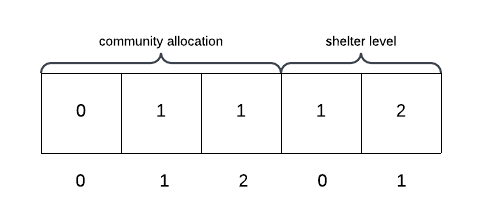
\includegraphics[width=250px]{Chromosome}
		\label{Chromosome}
	\end{figure}
	
	\textit{Population.} A group of chromosomes. This refers to a group of generated solutions on the problem that will be later on picked or selected.
	
	\textit{Generation.} A whole iteration process of genetic algorithm. This refers to the population on a certain generation which in theory, higher generations then the closer the user gets to the optimal solution.
	
	\textit{Fitness.} A value generated from the objective function. This refers to the objective value of a chromosome based on the implemented model.
	
	A genetic algorithm is composed of three key components: selection, crossover, and mutation. Each serves a distinct purpose in addressing optimization problems and simulates the evolution theory. Each component has various implementation methods tailored to specific objectives. \parencite{Eyal2020}
	
	\textit{Selection.} A process of selecting parents. This refers to selecting two chromosome based on their fitness value. The proposed system uses Roulette Wheel Selection, which is the likelihood of a chromosome to be selected is directly proportional to its fitness value. Figure \ref{Selection} shows that the probability is inversely proportional to the fitness value, since the researchers aim to minimize the objective. Moreover, a randomizer will select a chromosome based on the computed probabilities.
	
	\begin{figure}[h!]
		\caption{Selection process where probability is based on their fitness value.}
		\centering
		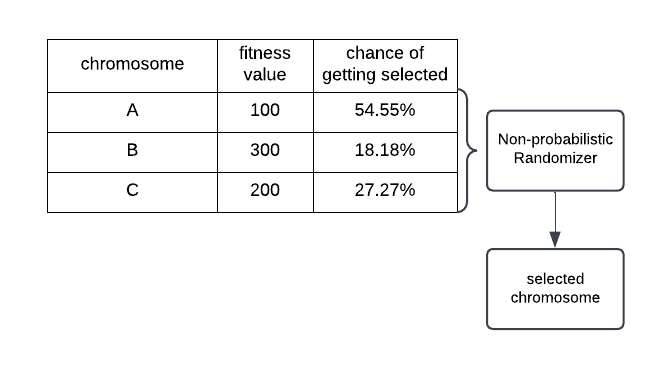
\includegraphics[width=350px]{Selection}
		\label{Selection}
	\end{figure}
	
	\textit{Crossover.} A process of breeding and giving offspring by a two parents. This refers to combining two selected chromosome values and generating a new chromosome based on the combined values. The proposed system uses Uniform Crossover, which all the values from two parents has a change to be inherited by the offspring. Figure \ref{Crossover} shows a generated offspring with values based on their parents. Notice that if a value is different between parents, a randomizer will decide which value would be chosen.
	
	\begin{figure}[h!]
		\caption{Crossover process where parents generate a new offspring}
		\centering
		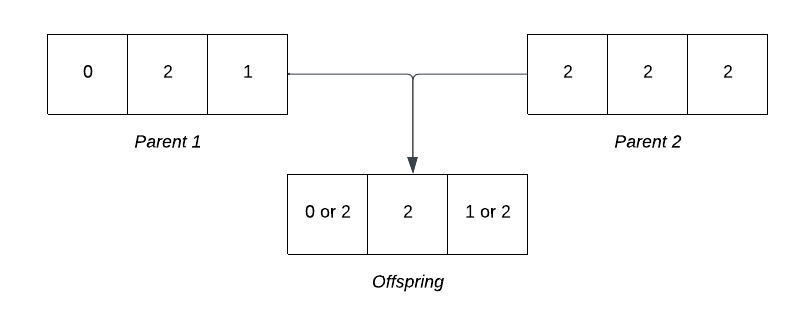
\includegraphics[width=350px]{Crossover}
		\label{Crossover}
	\end{figure}
	
	\textit{Mutation.} A process of altering some chromosome values. This refers to randomly selecting a chromosome from a population based on a predetermined mutation rate, then changing some of its values. The proposed system uses Random Reset Mutation, which picks randomly from a selected chromosome values, then changing it by generating a new random number. Figure \ref{Mutation} shows altering of a chromosome for the second community by a randomizer, allocating from shelter 1 to shelter 2.
	
	\begin{figure}[h!]
		\caption{Mutation process where a value is randomly altered}
		\centering
		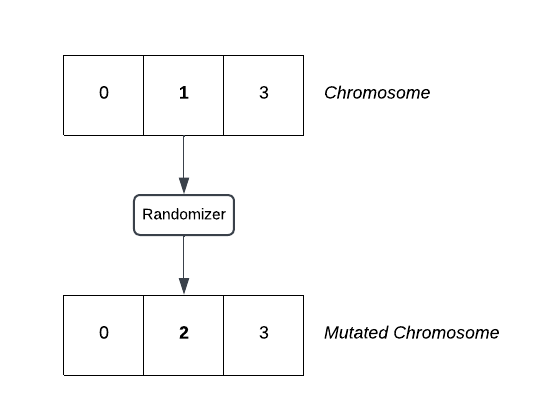
\includegraphics[width=300px]{Mutation}
		\label{Mutation}
	\end{figure}
	
	By applying these evolutionary principles, the genetic algorithm can efficiently navigate the large and complex problem space of shelter allocation, ensuring the most effective distribution of evacuees to shelters based on the model’s constraints and objectives.
	

	
	
\section{Process of Developing the System}
	This study employed a structured system development methodology following the Agile approach. Agile was chosen for its flexibility and iterative nature, which allows for continuous refinement and adaptation of the system based on feedback and testing results. Each development phase—planning, design, implementation, testing, and deployment—includes regular reviews and adjustments to ensure the system evolves effectively to meet technical and user needs.
	The system development process was divided into several distinct phases, each of which is designed to build upon the previous stage, ensuring a comprehensive and systematic approach. As shown in Figure \ref{Agile} originally illustrated by \textcite{Jayathilaka2020}

	\begin{figure}[h!]
		\caption{A representation of an Agile approach}
		\centering
		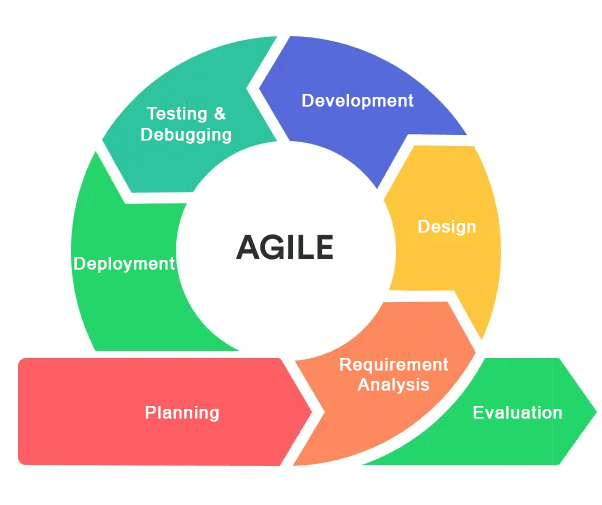
\includegraphics[width=0.6\textwidth]{AGILE}
		\label{Agile}
	\end{figure}

\subsection{Planning}

	In the initial phase, the researchers outlined the shelter location allocation system's scope, objectives, and requirements. This process identifies the key features and functionalities essential for the system. Additionally, this phase includes the thesis project plan, which details the project timeline.
	The Gantt chart outlines the phases of the thesis project, including thesis one output, thesis two output, data collection and preparation, paper miscellaneous, system design, system development, and system assessment. Each phase addresses specific objectives that contribute to completing the shelter location-allocation system. The Gantt chart is shown in Figure \ref{Gantt}.
	
	\textbf{Thesis One Output:} This phase involves drafting the initial sections of the thesis, such as the overview, rationale, scope, and significance, along with Chapters one through three (Introduction, Review of Related Literature, and Methodology). Additionally, this phase includes preparing the proposal manuscript, slides, and script for the mock defense and proposal defense. Parallel to this is the Paper Miscellaneous, which includes the creation of the literature review matrix to organize and support the contents of Chapter 2. This approach maintains a well-structured reference base for literature review.
	
	\begin{landscape}
		\begin{figure}[h]
			\caption{Gantt Chart}
			\centering
			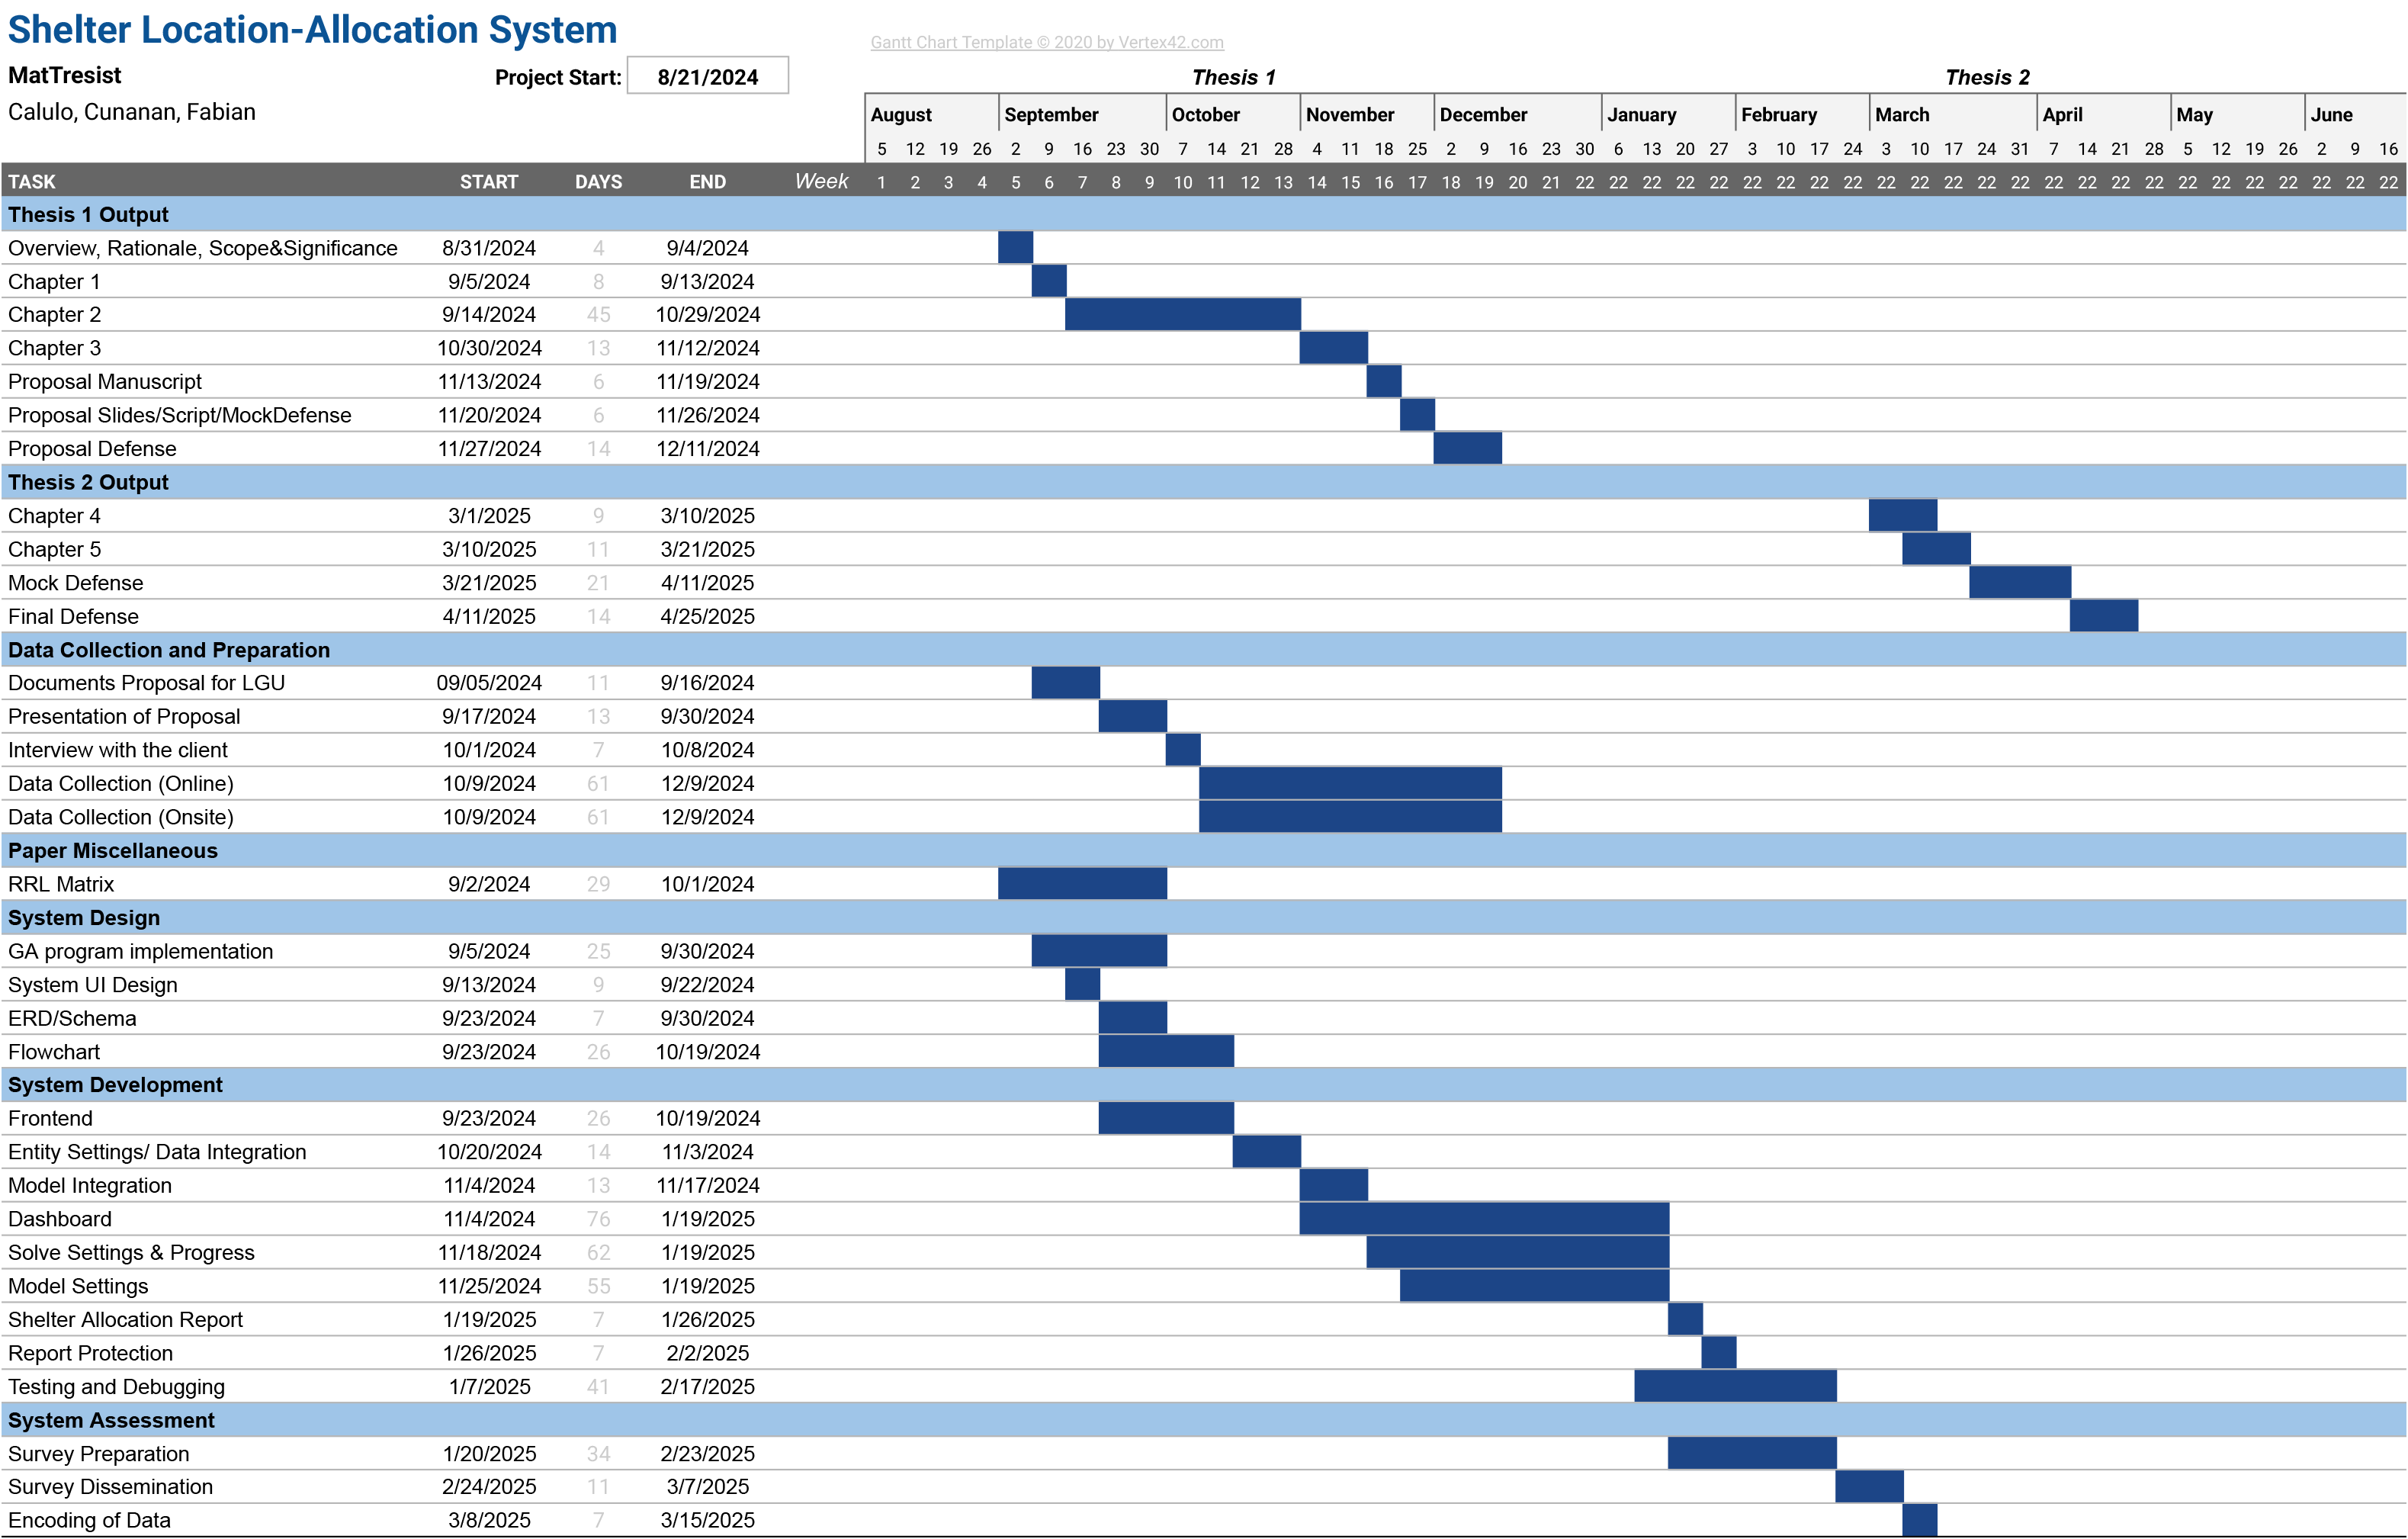
\includegraphics[width=600px]{Gantt}
			\label{Gantt}
		\end{figure}
	\end{landscape}
	
	\textbf{Thesis Two Output:} Following the foundational work in the first thesis phase, this continues the development of this thesis document, focusing on Chapters 4 and 5 (Results and Conclusions) and preparing for the mock defense and final thesis defense. This phase signifies the completion of the thesis writing process.
	
	\textbf{Data Collection and Preparation:} This critical phase entails gathering data required for system design and important data for the genetic algorithm. Tasks include submitting documents to the LGU, presenting the project proposal, conducting client interviews, and collecting online and onsite data.
	
	\textbf{System Design:} This phase focuses on planning the technical aspects of the shelter allocation system, including genetic algorithm implementation, user interface design, entity relationship diagram, and flowchart development. These elements form the blueprint that guides the system's development.
	
	\textbf{System Development:} The project's core phase involves the actual construction and coding of the system. Tasks include front-end development, data and model integration, dashboard creation, and implementing security features. This phase also includes testing and debugging to ensure system functionality.
	
	\textbf{System Assessment:} The final phase, along with Thesis Two Output, is evaluating the system's acceptability and user satisfaction. Activities include preparing and distributing surveys, gathering user feedback, encoding and analyzing this data to assess system acceptability.

\subsection{Requirement Analysis}
	During the requirement analysis phase, researchers gathered comprehensive information about the system requirements by reviewing relevant literature that pertains to the thesis. Moreover, an interview with the client was conducted to know more about the current issues LGUs are facing regarding to evacuation. This phase ensures that all necessary features are identified and prioritized based on their importance.
	
	The system's primary features and requirements encompass an overview of data and model modification, data simulation, shelter tagging, and report protection. Data modification includes an access to user for managing and modifying community and shelter data. Model modification allows users to change parameters on data simulation.Data simulation utilizes the community and shelter data as inputs for the genetic algorithm applied in the shelter location allocation system, optimizing the placement of evacuees in shelters. Furthermore, shelter tagging enables the categorization of shelters based on criteria such as location, capacity, and suitability for various disaster scenarios, thereby facilitating efficient resource allocation. Lastly, report protection allows user to protect their generated report to prevent leaks in a computer system.
	
\subsection{Design}
	During the design phase, the researchers created a detailed outline for the shelter location-allocation system's architecture and key components. The design process includes creating a mockup of the system's user interface and constructing flowcharts, an entity-relationship diagram (ERD), and a data flow diagram(DFD) to map out system processes and data relationships. The researchers designed mockups to visualize the user interface, ensuring it met the user's needs for accessibility and usability. The flowcharts provided a step-by-step breakdown of system processes, while the ERD defined the data structures and relationships. These elements formed a cohesive blueprint to guide the system's development and ensure alignment with the requirements. Figure \ref{SystemArch} shows the system architecture which combines DFD and the interaction of users.

	\begin{figure}[h!]
		\caption{System Architecture}
		\centering
		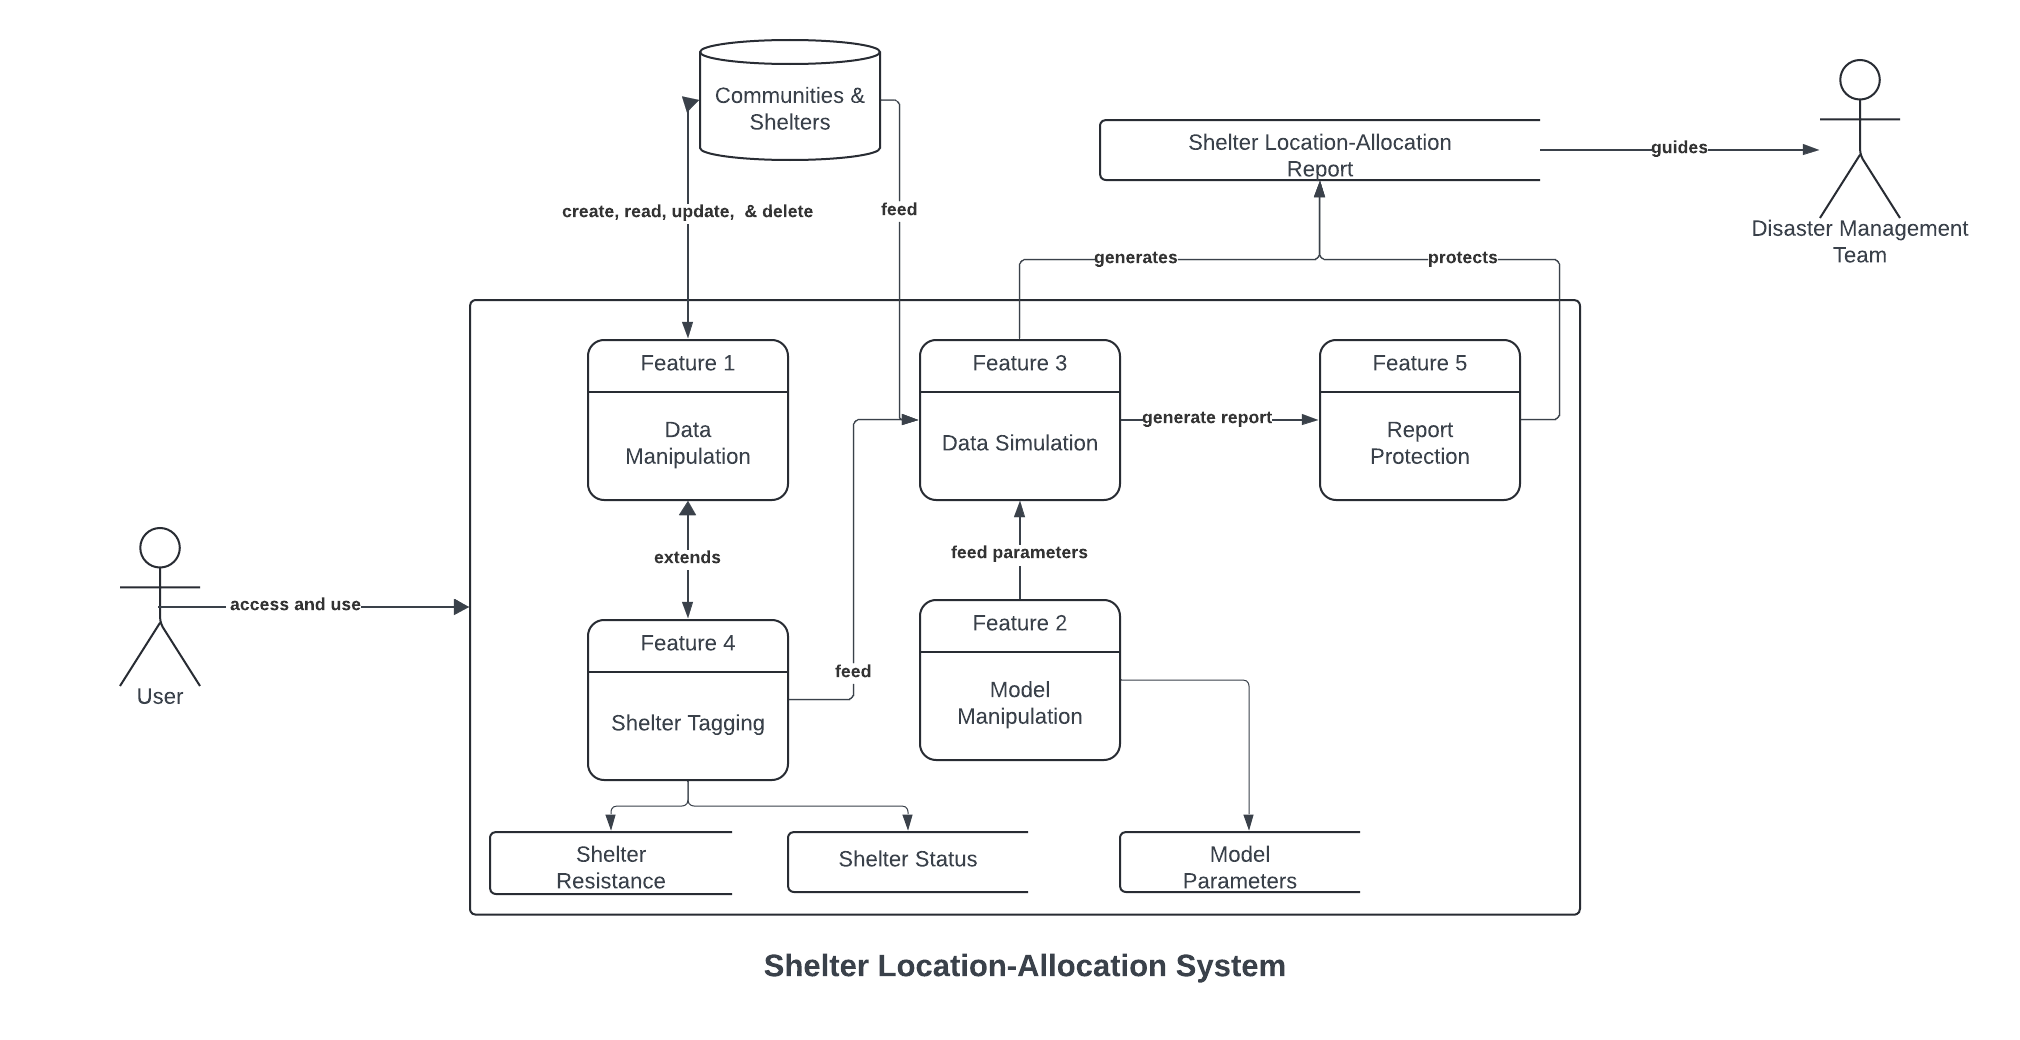
\includegraphics[width=\textwidth]{Context Diagram}
		\label{SystemArch}
	\end{figure}
	
	The system architecture involves the interaction of two actors, the user of the system and disaster management team. The community and shelter data will be fed into a system which features data manipulation and shelter tagging. With the cleaned or finished data, data simulation may begin together with the model parameters modified by the user. Finally, a report will be generated and can be protected or not. The report will be used by the disaster management team to guide them for decision making in allocation of residents to the correct shelter.

	\begin{figure}[h!]
		\caption{The ERD Schema}
		\centering
		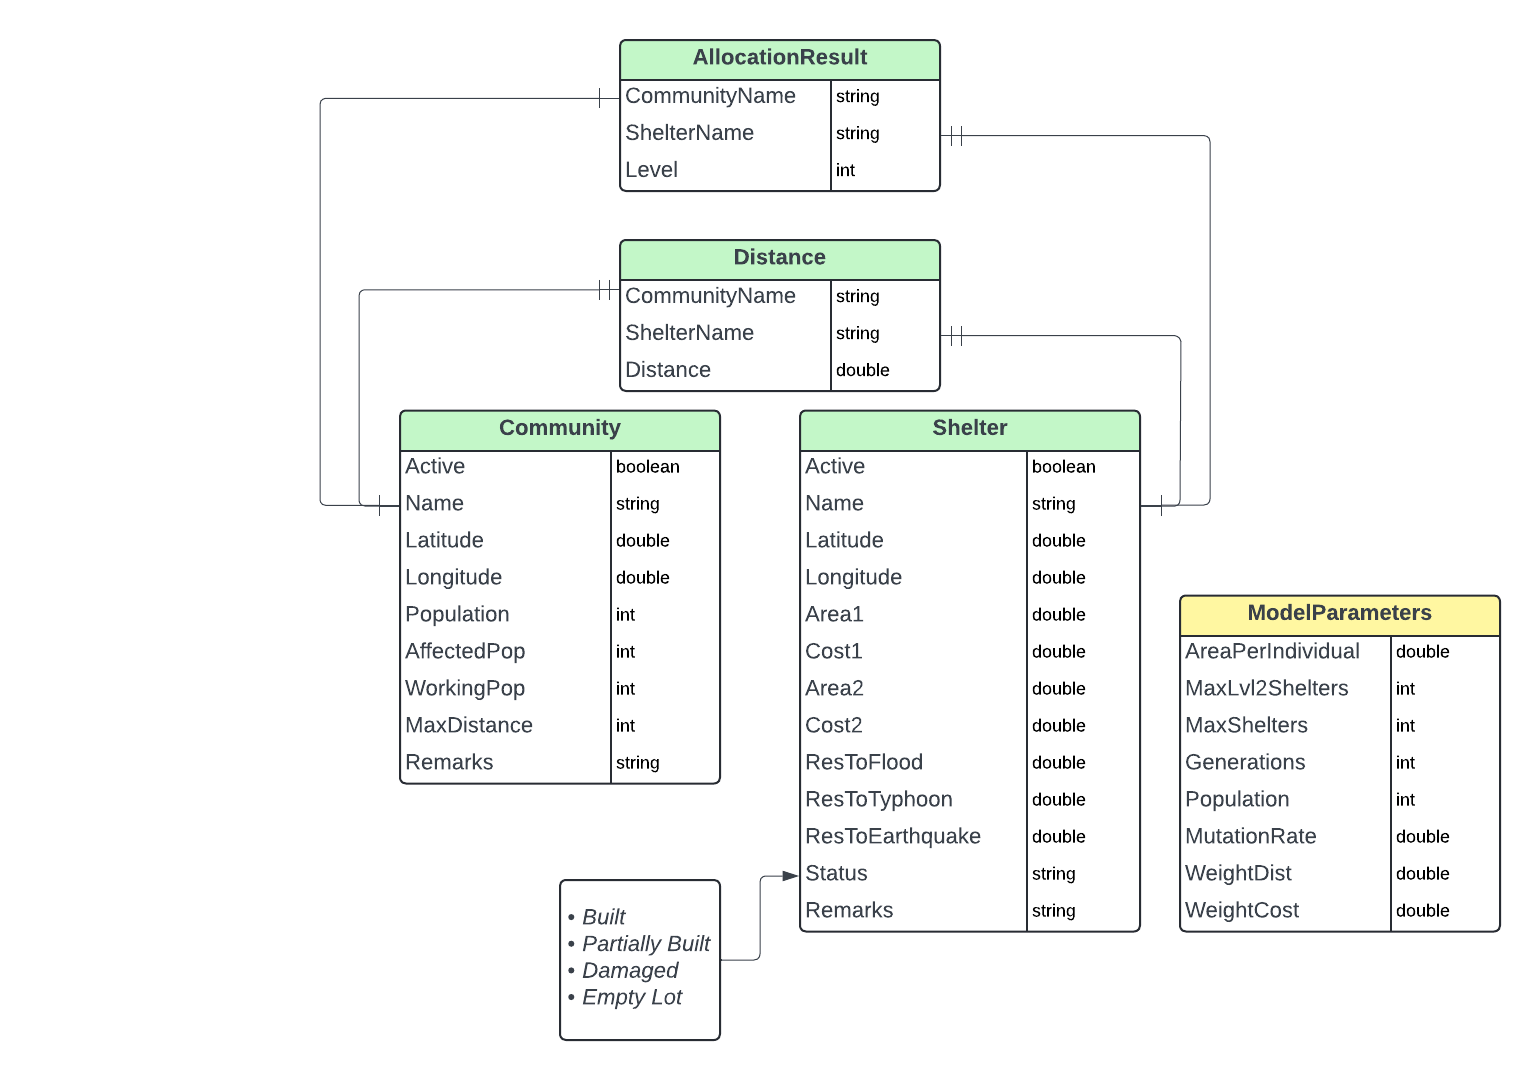
\includegraphics[width=\textwidth]{ERD}
		\label{ERD}
	\end{figure}
	
	Figure \ref{ERD} shows the entity relationship (ERD) which has 4 entities: Community, Shelter, Distance, and ModelParameters. Distances are derived from the location of Shelter and Community, then will be saved accordingly to be used in performing the system model. ModelParameters shows no relationship since it only saves the current settings for the model and algorithm.
	
	A system mock-up was made showing the prototype of the system by designing the User Interface (UI) using a prototyping tool, Figma. The mock-up shows the UI for different modules of the system.

\subsection{Development}
	The development phase includes coding and implementing the genetic algorithm for the shelter location allocation system. Utilizing the Agile system development life cycle, which includes weekly meetings and development reviews, the team can ensure that development remains on track and that any issues are promptly addressed. By following the Agile SDLC, the researchers can adapt quickly to any changes in requirements, maintain clear communication, and address any issues promptly.
	
	Table \ref{TechUsed} shows the list needed to start the development process. The system was developed using Python programming language, and Qt framework to efficiently implement the graphical user interface(GUI) of the system. Visual Studio Code was utilized as the integrated development environment (IDE), and QtDesigner as an extension for creating frontend designs by Qt framework.
	
	\begin{table}[h]
		\centering
		\caption{List of tools and technologies used in the development process}
		\label{TechUsed}
		\renewcommand{\arraystretch}{1.3}
		\resizebox{\textwidth}{!}{
			\begin{tabular}{llp{8cm}}
				\hline
				\multicolumn{1}{l}{\textbf{Name}} & 
				\multicolumn{1}{l}{\textbf{Version}} & 
				\multicolumn{1}{l}{\textbf{Description}} \\ \hline
				Visual Studio Code   & 1.96.3   & IDE for the whole coding and debugging process            \\ 
				Python               & 3.12.5   & Programming language known for extensive computation libraries  \\ 
				QtDesigner           & 5.11.1   & GUI design tool which has drag and drop feature \\ 
				GitKraken            & 10.6.1   & Git client that is user friendly for executing Git commands      \\ 
				GitHub               & Web      & Repository host which used for collaboration and backup of the project\\ \hline
			\end{tabular}
		}
	\end{table}
	
	Developing the proposed system using Python allows us to use Python libraries. As shown in Table \ref{PythonUsed}, displays all the libraries used to develop the system. PySide6 is responsible for the GUI that uses the Qt framework. Pandas and openpyxl are used for handling data. Folium, OSMnx, networkx, and scikit-learn are for displaying and calculating the map shown in the system. Numpy is used for executing genetic algorithm. Additionally, msoffcrypto-tool and XlsxWriter are used for report protect and lastly, pyinstaller for building the system.
	
	\begin{table}[h]
		\centering
		\caption{List of libraries installed in Python}
		\label{PythonUsed}
		\renewcommand{\arraystretch}{1.3}
		\resizebox{\textwidth}{!}{
			\begin{tabular}{llp{8cm}}
				\hline
				\multicolumn{1}{l}{\textbf{Name}} & 
				\multicolumn{1}{l}{\textbf{Version}} & 
				\multicolumn{1}{l}{\textbf{Description}} \\ \hline
				PySide6   & 6.7.2   & Uses Qt framework for frontend development \\ 
				pandas               & 2.2.3   & Reads and handles datasets  \\ 
				openpyxl            & 3.1.5   & Opens and reads excel files \\ 
				folium            & 0.17.0   & Provides visualization and interactivity on a geographical map  \\ 
				osmnx               & 1.9.4      & Retrieves OpenStreetMap(OSM) data and could calculate road paths\\ 
				networkx               & 3.3      & Creates and computes complex graphs such as road networks\\ 
				scikit-learn               & 1.5.2      & Provides simple machine learning tools and functions\\ 
				numpy               & 1.26.4     & Generates non probabilistic numbers \\ 
				msoffcrypto-tool & 5.4.2     & Encrypts and decrypts excel files \\ 
				XlsxWriter & 3.2.2     & Edits and writes excel contents \\ 
				pyinstaller & 6.12.0     & Compiles project file into an executable file \\ \hline
				
			\end{tabular}
		}
	\end{table}
	
	
	
\subsection{Testing and Debugging}
	The system underwent functionality, performance, and reliability testing during the testing phase. The researchers employed manual testing techniques to identify and resolve any bugs or issues that arise. Any errors and anomalies found in the system are debugged and fixed. Through this thorough testing and debugging approach, the researchers ensure that the shelter location allocation system meets high quality, performance, and user satisfaction standards, making it ready for deployment.
	
\subsection{Deployment}
	During the deployment phase, the shelter location-allocation system underwent pilot testing in collaboration with local government units (LGUs). This process involved configuring the system, establishing the necessary data inputs, and training users to utilize the platform effectively. Additionally, the deployment phase is to continuously monitor the system's performance to ensure it operates efficiently and meets the objective of optimizing shelter locations. 

	Presentation of the application to the potential users, specifically the LGU of Calumpit include a walk-through tutorial covering all essential features. The users was provided with the information necessary to operate the app effectively, including an overview of its purpose, functionalities, and how to input relevant data. Specifically, this includes entering shelter locations, population data, and accessibility metrics into the system to ensure accurate allocation results. Since a detailed explanation was provided during the system evaluation, this presentation focused on summarizing key points and addressing questions and feedback from the users.
	
\subsection{Evaluation}
	Evaluation of the system includes preparing any distributing survey questionnaires based on TAM and ISO/IEC 25010 to our target sample. This phase ensured that the developed system has feedback from potential users as well as from experts in software engineering and development.
	
	Feedback gathered from the potential users were important in identifying the areas for improvement. This feedback was collected through structured surveys and interviews to provide a comprehensive understanding of user needs and challenges. After the updates and adjustments to the application based on feedback to better align with users’ needs, the new version of the application has been emailed to the LGU of Calumpit for operational use. This ensured that they have access to the latest features and improvements. It is important to note that this application is copyrighted by Bulacan State University to protect its intellectual property and ensure proper recognition to the researchers, developers, and thesis adviser. This copyright also prevents unauthorized commercial use and distribution, ensuring that the application remains a free resource for its intended purpose. It is not for sale.

\section{System Preliminaries}
	Developing a system requires careful planning and analysis before implementing it. A communication between the potential users or clients and the researchers is essential to ensure all system requirements are met and improved. This phase aims to establish a foundational understanding of current disaster-response processes, along with gathering essential data for the system. Interviews was conducted with representatives from local government units (LGUs) specifically from the target population to understand their existing shelter allocation process, challenges, and expectations for a decision support system. 
	
\subsection{Client Interview}
	Conducting an interview with the client is essential to get to know with the potential users and the problems their facing. Questions formulated are derived from Design Thinking Framework which is according to \textcite{Julio2018} has resulted a greater approximation of end users and the development team who uses an Agile SDLC. This improves the quality and usability of the software.
	
\subsection{Data Gathering}
	The model needed data to perform, specifically community and shelter data. Additionally, to ensure that the system produces outputs, data on shelters, disaster events, and typhoons were collected. This includes accessing records on past typhoon impacts, available shelter locations, and their respective capacities. Community or barangay data was sourced from publicly available databases, such as PhilAtlas, which provides detailed geographical and demographic information essential for accurate system modeling.
	
\subsection{Data Preprocessing}
	The gathered information has undergone several stages. This ensures it meets the needs of the system and allows for an accurate assessment of its effectiveness.
	
	All collected data were first cleaned to remove any inconsistencies, duplicates, or irrelevant information. This process is crucial for ensuring the data’s quality and reliability, particularly for a system that relies on precision in both inputs and outputs. Any insufficient data was asked to the LGU to fill in the gaps of the datasets. 
	
	Table \ref{dataSource} presents all the data variables on communities and shelters used in the model, along with their respective sources. Affected population were derived from the population of community which is based on the study of \textcite{Opdyke2024} that states 12\% of households intends to evacuate on public evacuation sites. Improvement or rehabilitation cost is added for costs, which are based on a report for improvement of an evacuation center from \textcite{DilgL1area2022,DilgL1cost2022} that costs approximately ₱7,700 per square meter. Meanwhile, data for Level 2 shelters are simulated, as the LGU does not have a data nor system for the hierarchy of shelters. The areas are assumed to be twice their initial size, and costs are estimated based on the contract cost of the Frances Evacuation Center, as detailed in the \textcite{DilgL22022,Dpwh2022} reports, resulting in approximately ₱60,000 per square meter. 
	
	\begin{table}[h]
		\centering
		\caption{Variables, Descriptions, and Sources for Community and Shelter Data}
		\label{dataSource}
		\renewcommand{\arraystretch}{1.3}
		\resizebox{\columnwidth}{!}{
			\begin{tabular}{lp{6cm}p{9cm}}
				\hline
				\textbf{Variable} & \textbf{Source} & \textbf{Description} \\ \hline
				\multicolumn{3}{l}{\textit{Community}}\\ 
				Name & LGU interview & Identity of a community \\ 
				Longitude & Google Map \& LGU interview & Longitudinal coordinates \\ 
				Latitude & Google Map \& LGU interview & Latitudinal coordinates \\ 
				Population & Philippine Atlas (2020 population) & Number of individuals living in a community \\ 
				AffectedPop & Assumed 12\% of Population & Number of individuals affected during a disaster \\ 
				MaxDistance & Maximum distance generated in distance calculation & Distance allowed to travel by a community \\ 
				\multicolumn{3}{l}{\textit{Shelter}} \\ 
				Name & LGU interview & Identity of a shelter \\ 
				Longitude & Google Map \& LGU interview & Longitudinal coordinates \\ 
				Latitude & Google Map \& LGU interview & Latitudinal coordinates \\ 
				Area1 & Google Map & Lot area of a shelter (level 1) \\ 
				Cost1 & Assumed 7,700 * Area1 & Cost for constructing/maintaining a shelter with Area1 \\ 
				Area2 & Assumed Area1 * 2 & Lot area of a shelter (level 2) \\ 
				Cost2 & Assumed 60,000 * Area1 & Cost for constructing/maintaining a shelter with Area2 \\ 
				ResToFlood & LGU interview & Resistance to flood indicator \\ 
				ResToTyphoon & LGU interview & Resistance to typhoon indicator \\ 
				ResToEarthquake & LGU interview & Resistance to earthquake indicator \\ 
				Status & LGU interview & State of the physical structure of a shelter indicator \\ 
				\multicolumn{3}{l}{\textit{Distance between Community and Shelter}} \\ 
				distance & OpenStreetMap API & distance needed to travel by a community to a shelter  \\ \hline
			\end{tabular}
			}
	\end{table}
	
	Researches added empty lots across Calumpit to be appended to shelter data. These lots are identified and selected to be resistant to hazards, specifically floods with the assistance of Nationwide Operational Assessment of Hazards (NOAH) website. Table \ref{AppendData} shows the change of variables in area, cost, resistance and status for these appended shelter data. Additional cost is added due to property cost which according to Dot Property, approximately ₱12,500 per square meter was the average cost for land in Calumpit.
	
	\begin{table}[h]
		\centering
		\caption{Sources of Appended Shelter Data}
		\label{AppendData}
		\renewcommand{\arraystretch}{1.3}
		\begin{tabularx}{\textwidth}{>{\raggedright\arraybackslash}p{4cm} X}
			\hline
			\textbf{Variable} & \textbf{Source} \\ \hline
			Cost1            & Assumed Area1 * (60,000 + 12,500) \\ 
			Cost2            & Assumed (Area2 * 60,000) + (Area1 * 12,500) \\ 
			ResToFlood       & Assumed TRUE \\ 
			ResToTyphoon     & Assumed TRUE \\ 
			ResToEarthquake  & Assumed TRUE \\ 
			Status           & Already an Empty Lot \\ \hline
		\end{tabularx}
	\end{table}
	
	For justification of the target area’s vulnerability, typhoon data spanning from 2006 to 2022 were examined. This dataset includes the number of affected and evacuated individuals across various municipalities in Bulacan. The data was grouped by municipality, summing the affected and evacuated residents over the specified period. This analysis helps justify the focus on the municipality and supports the rationale for the shelter allocation model’s implementation in the municipality.
	
	The cleaned shelter and community data were fed into the system to facilitate accurate shelter location-allocation modeling. The system will use these inputs to generate optimized shelter placement recommendations based on the model adopted.
	
	
\section{System Evaluation}
	System evaluation focuses on assessing acceptability of the shelter location allocation system using the TAM determinants and ISO/IEC 25010 standard. These standards provides a framework for evaluating the software's quality and acceptability. The system evaluation includes the evaluation instrument, determining the population and sample, outlining data collection procedures, and discussing the data analysis techniques used.

\subsection{Evaluation Instrument}
	The evaluation instrument is a structured questionnaire designed to assess the acceptability of the shelter location allocation system based on the determinants of Technology Acceptance Model(TAM) and key quality attributes outlined in the International Organization for Standardization and International Electoral Commission (ISO/IEC) 25010 standard. Questionnaires based on TAM was distributed to the potential end-users of the system. On the other hand, questionnaires based on ISO/IEC 25010 was distributed to the experts in software development.
	
	TAM questionnaire evaluates the system's acceptability by the user of the system. This model answers why users accept or reject information systems, and examines a system's acceptance based on their attitudes, preferences, and behaviors.\parencite{Davis1987}
	\\The following criteria are based upon the four determinants defined in TAM:
	\begin{enumerate}
		\item \textit{Perceived Usefulness.} This answers on how much a user believes using the system will improve their performance such as job tasks. It evaluates whether the users thinks the proposed system will be genuinely beneficial to LGUs or if it can assist other LGUs effectively.
		
		\item \textit{Perceived Ease of Use.} This answers on how much a user believes using the system will be efficient and user-friendly. It considers whether the proposed system can be used smoothly with minimal errors and without performance issues.
		
		\item \textit{Attitude Towards Using.} This answers on what user feels when using the system based on their enjoyment and satisfaction. A positive attitude towards the system often leads to accepting the technology.
		
		\item \textit{Behavioral Intention to Use.} This answers on willingness to use the system in the future. It determines whether users find the system valuable enough to incorporate into their long-term plans.
	\end{enumerate}
	
	
	Additionally, ISO/IEC 25010 questionnaire evaluates various aspects of the system, including usability, reliability, performance efficiency, and overall user satisfaction. Through this instrument, the study aims to gather objective data that will help determine how well the system meets user needs and expectations. \parencite{ISOIEC2023}
	\\The following criteria are based upon the nine quality characteristics for product quality model defined in ISO/IEC 25010:
	
	\begin{enumerate}
		\item \textit{Functional Suitability.} This evaluates how well the system meets user needs and performs its intended functions. The questions will focus on the system's ability to allocate shelters effectively, manage community and shelter information, and provide accurate data.
		
		\item \textit{Performance Efficiency.} This attribute will evaluate the system's response time and processing capacity. The questionnaire will include items assessing the system's speed in performing functions, efficient use of resources such as memory and processing power, and ability to handle maximum load requirements. By examining performance efficiency, the study aims to determine whether the system can perform reliably under diverse operational conditions.
		
		\item \textit{Compatibility.} This will assess the system’s ability to exchange and use information with other systems. The questionnaire will ask how well the system integrates with external databases, applications, or computer systems. 
		
		\item \textit{Interaction Capability.} This will prioritize the system's usability, learnability, and overall user satisfaction. The questionnaire will gather detailed user feedback regarding their experiences with the system. The questionnaire will address aspects such as ease of navigation, effectiveness in completing tasks, and general user engagement.
		
		\item \textit{Reliability.} This attribute will assess the system's interaction capability, focusing on its ease of use, appropriateness for users, and ability to guide users in completing tasks effectively. The evaluation will include questions on how easily users can recognize if the system meets their needs, learn its functions, and operate it with minimal errors. Additional focus will be on user engagement, inclusivity, and the availability of assistance to support a diverse range of users. 
		
		\item \textit{Security.} The system ensures that all collected data will remain confidential and solely for this research. No data will be uploaded online, and all information will be stored offline. Access to data will be limited to the researchers and users.
		
		\item \textit{Maintainability.} This will evaluate the system's ease of adaptability to meet new requirements, correct errors, and improve performance. The questionnaire will assess the system's reusability, analyzing how parts of the system can be leveraged in future developments or other systems, and its testability, ensuring that any necessary changes can be efficiently implemented and quickly identified so that testing can be done efficiently. 
		
		\item \textit{Flexibility.} This will assess the system’s ability to adapt to changing user needs and requirements. The questionnaire will evaluate the system's ability to support new features, incorporate updates, and seamlessly integrate with additional tools or systems as necessary. It will also examine how well the system accommodates changes in shelter allocation criteria, such as shifts in population density and shelter resistance.
	\end{enumerate}
	

\subsection{Population and Sample}
	The population of this study consists of end-users and IT experts. For end-users,  MDRRMO and MSWDO of the municipality of Calumpit. Meanwhile for IT experts, includes CICT professors from Bulacan State University, and someone who have experience in developing a system.  The diversity of perspective of these are important for the comprehensive evaluation of the system’s acceptability.
	
	\textbf{MDRRMO:} The staff consists of Municipal Disaster Risk Reduction Management Office (MDRRMO), who are responsible for formulating and implementing the province's disaster risk reduction plan.  Their insights are vital for understanding the operational requirements considerations for implementing the shelter location allocation system, ensuring it aligns with established disaster response protocols and local needs.
	
	\textbf{MSWDO:} The Municipal Social Welfare and Development Office (MSWDO) plays a key role in managing the evacuation and welfare of the communities during disasters. Their expertise is essential in ensuring that the shelter allocation system aligns with evacuees' specific needs, such as accessibility and capacity to the shelter location allocation across the province. Their input assisted tailoring the system to address the welfare requirements of evacuee management during emergencies.
	
	\textbf{CICT professors:} Coming from the College of Information and Communication Technology (CICT) of Bulacan State University, professors have significant academic background and experience to technologies. This part of population assessed the system's performance and functionality with the help of their knowledge and expertise.
	
	\textbf{System Developers:} Experts with extensive experience in system development play an important role in project evaluation. They are commonly found in businesses that design, propose, and develop systems for their clients. Their expertise enables them to understand and address real-world client requirements, guiding the system to be acceptable to users.
	
	The sampling technique that was utilized for end-users is Stratified Sampling Technique, where the population is divided into a respective groups or strata, where in this study, our stratum is the MDRRMO and MSWDO. This ensures comprehensive representation, to capture the perspectives of different stakeholder groups proportionately. The sample size of end-users were then computed using G*Power, a statistical software tool. With a confidence level of 95\% or 0.05 margin of error, the sample size would be 23. Since the sample size would be much smaller than the population size, then conducting system evaluation would be feasible.
	
	Meanwhile, for IT experts, Purposive Sampling Technique was employed. Researchers purposively selected 5 IT experts. These experts was chosen based on their qualifications and relevant experience to provide insights into the system's design, functionality, and performance. This technique ensured that the selected experts evaluating the system provided comprehensible and accurate feedback while also ensuring its feasibility.
	
\subsection{Data Collection Procedures}
	Evaluation phase gauges the system’s acceptability and user satisfaction. To do this, a questionnaire was developed based on TAM and ISO/IEC 25010, which employs a 10-point rating scale, allowing participants to provide precise feedback on each quality criterion. The system was demonstrated to a selected sample population in a face-to-face presentation, where they had the chance to interact with the system firsthand. This was followed by the completion of the questionnaire, enabling participants to provide feedback based on their experience using the system.
	
	Following the research instruments ensures that the system meets its intended objectives and offers insights into potential areas for improvement, which were critical for broader implementation in disaster-response operations. Through the data collection process, the researchers ensured that all ethical considerations are thoroughly addressed to uphold the integrity and privacy of the participants

\subsection{Data Processing and Analysis}
	This study's data processing involves structured analysis to interpret findings from the acceptability survey, aligning with the ISO/IEC 25010 standard and TAM determinants. This standard evaluates key quality attributes, and each attribute was assessed using a 10-point numerical rating scale. 1 = completely disagree, and 10 = completely agree, as shown in Figure \ref{Nrs}
	
	\begin{figure}[h!]
		\caption{10-point numerical rating scale}
		\centering
		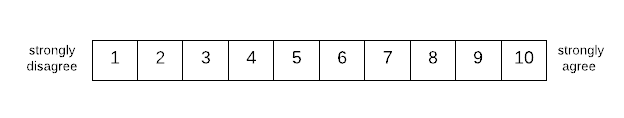
\includegraphics[width=3.5in]{Nrs-10}
		\label{Nrs}
	\end{figure}
	
	After the data collection, the rating scale categorizes the acceptability levels. Descriptive statistics was utilized to analyze the collected data. Analysis includes calculating the minimum, maximum, mean, and standard deviation for each category.
	
	\begin{equation*} 
		\label{mean}
		\bar{x} = \frac{\sum_{i=1}^{n} x_{i}}{n}
	\end{equation*}
	
	\noindent where: \\
	\begin{tabular}{@{}ll}
	$\bar{x}$ & sample mean \\
	$n$ & sample size \\
	$x_{i}$ & data points \\
	\end{tabular}
	
	\noindent shows the mean that computes the average score. This use of data allows both the system functionality and its user acceptability to be comprehensively assessed. The following shows the verbal interpretation of the computed mean corresponds to the level of acceptability based on the study by \textcite{Eladia2024}:
	
	
	\begin{table}[h]
		\centering
		\renewcommand{\arraystretch}{1.3}
		\label{Verbal}
			\begin{tabular}{ll}
				\multicolumn{1}{l}{\textbf{Mean Score Interval}} & 
				\multicolumn{1}{l}{\textbf{Level of Acceptance}} \\ \hline
				1.00 - 2.80     & Poorly Acceptable            \\ 
				2.81 - 4.60     & Fairly Acceptable  \\ 
				4.61 - 6.40     & Acceptable \\ 
				6.41 - 8.20     & Moderately Acceptable      \\ 
				8.21 - 10.00    & Highly Acceptable\\ 
			\end{tabular}
	\end{table}
	
	
	\begin{equation*} 
		\label{stdDev}
		S = \sqrt{\frac{\sum_{i=1}^{n} (x_{i} - \bar{x} )^2 }{n-1}}
	\end{equation*}
	
	\noindent where: \\
	\begin{tabular}{@{}ll}
	$S$ & sample standard deviation \\
	$\bar{x}$ & sample mean \\
	$n$ & sample size \\
	$x_{i}$ & data points \\
	\end{tabular}
		
	\noindent shows the standard deviation calculation which shows the dispersion of scores relative to the mean. A standard deviation  that is closer to the value of 0 indicates the spread of data is closer to the mean.


\section{Ethical Considerations}
	Data gathered contained sensitive data so that ethical considerations should be practiced throughout the research.  Informed consent obtained from each participant, providing them with a clear understanding of the research purpose, procedures, and their rights to withdraw at any time. To protect the participants’ privacy, all responses are anonymized and handled with strict confidentiality. Additionally, data usage was restricted to research purposes only, ensuring that participants' information remains safeguarded throughout the research process and beyond. 
	
	\textbf{Informed Consent:} All respondents are informed about the purpose, procedures, and potential impacts of the study before they agree to participate. The respondents were given a detailed explanation of the study, including the nature of their involvement, the voluntary nature of participation, and their right to withdraw at any time.
	
	\textbf{Confidentiality and Anonymity:} Personal identifiers are removed from the data to ensure that the respondents cannot be traced back to other respondents. Data are stored securely, and access is restricted to the researchers. Any publications or presentations resulting from the study will use aggregated data with no individual responses disclosed, safeguarding the identity and privacy of all respondents.
	
	\textbf{Data Protection:} The study adheres to relevant data protection regulations, such as local data protection laws, ensuring the secure handling and storage of all collected data. Informing the respondents about how their data was collected, stored, and used. Their rights to privacy and data protection is respected, and only authorized researchers will have access to the information.
	
	\textbf{Minimizing Harm:} The study is structured to minimize any potential harm to respondents. This includes ensuring that all questions are respectful, non-discriminatory, and that the data collection process does not inconvenience the respondents. Any potential risks are clearly communicated, and measures are implemented to mitigate these risks and uphold the respondents well-being throughout the study.
	
	\textbf{Transparency and Honesty: } The researchers uphold transparency and honesty throughout every stage of the study. This commitment includes accurately reporting research findings, acknowledging limitations, and strictly avoiding data manipulation or bias. Respondents were informed of the study's progress, purposes, and outcomes, ensuring they remain fully aware of how their contributions are utilized and valued within the research.
	
	By adhering to these ethical principles, the study safeguards respondents' rights and well-being, uphold the integrity of the research process, and enhance the credibility and reliability of its findings. This ethical approach shows trust between researchers and respondents, contributing to meaningful and responsible research outcomes.
